\NEW{
\section{\newname: Real-time and Dynamic Bandwidth Separation with Online Traffic}
\label{sec:dynamic}

\begin{figure}[t]
  \centering
  %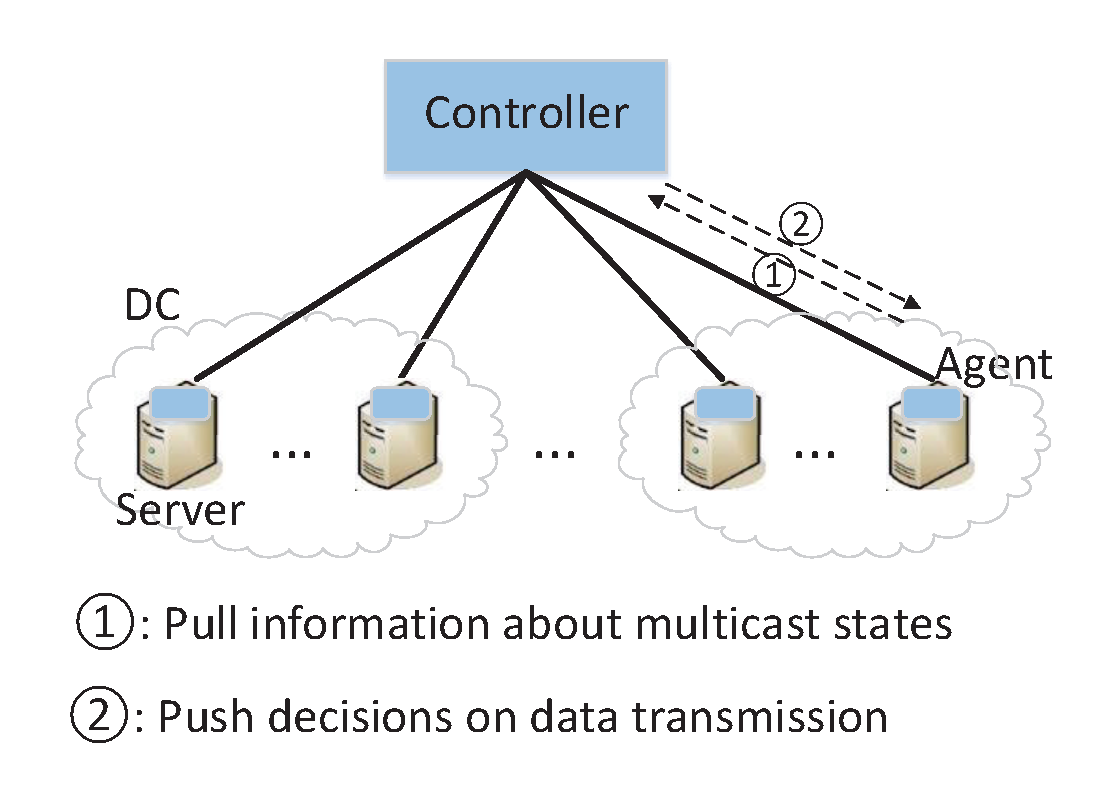
\includegraphics[width=2in]{images/framework.eps}
  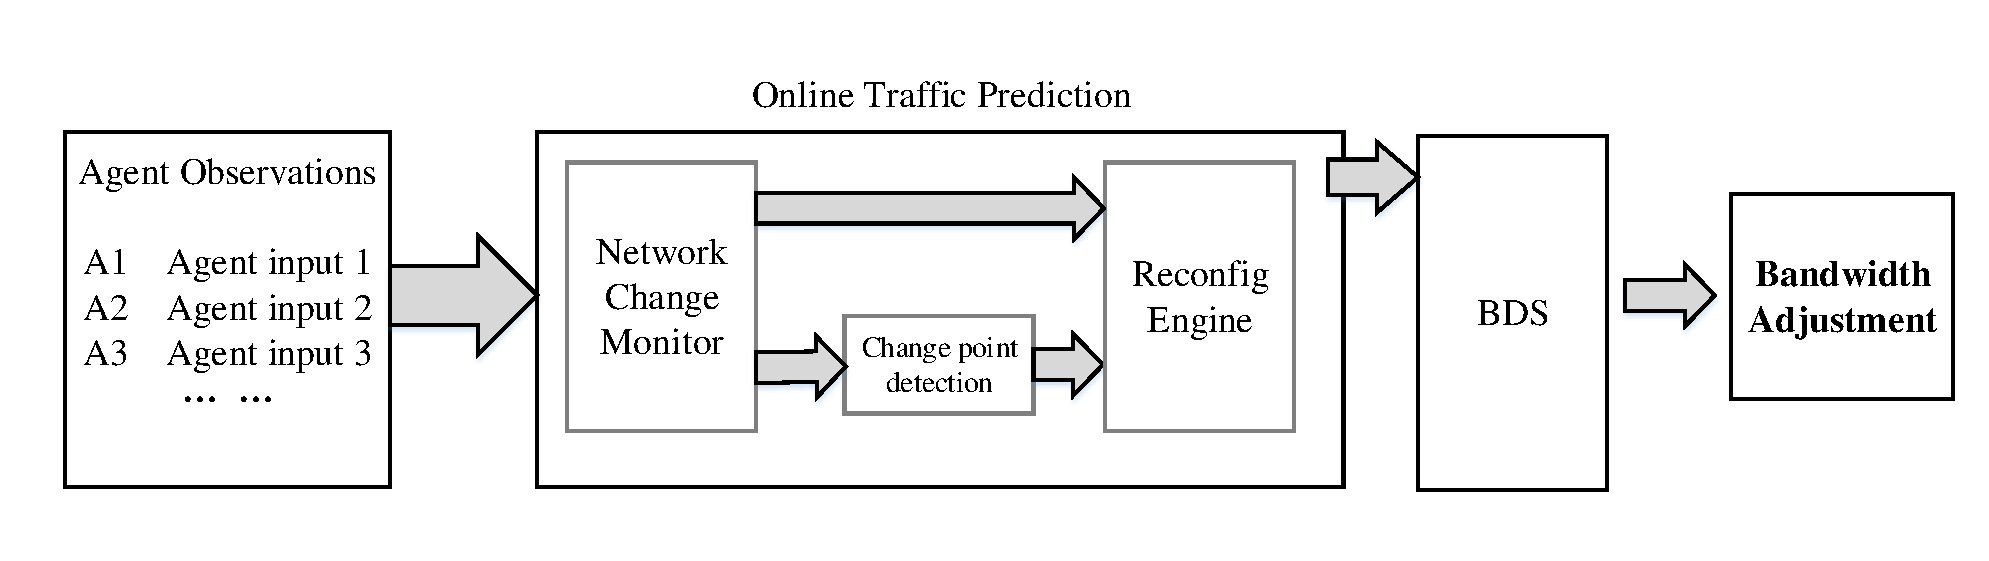
\includegraphics[width=3.4in]{images/Bayes.pdf}
    \vspace{-0.2cm}
  \tightcaption{\NEW{Logical diagram of \newname's online prediction.}}
  \label{fig:bayes}
\vspace{-0.4cm}
\end{figure}

\name performs well under strict network limitations, but sometimes results in poor bandwidth utilizations because the static \name bandwidth allocation algorithm {\em has limited dynamic range}: it will not occupy any more bandwidth even when online traffic is in the valley, because there is a strict safety threshold for bulk data transfer to avoid excessive link utilization (\Section\ref{subsec:motivation:baseline}).

In this section, we present an enhanced version of \name, called \newname, which achieves dynamic bandwidth separation with online traffic in a real-time manner, by continuously predicting online traffic changes and automatically adjusting the scheduling decisions to fully utilize network bandwidth accordingly. Thus, \newname automatically adjust the scheduling results under different network conditions: if online traffic encounters its peak, \newname would shirk its occupies bandwidth to avoid congestions, while online traffic encounters ite valley, \newname would aggressively use more bandwidth to fully utilize netwrok.

To achieve this, \newname uses an online traffic prdiction algorithm, which identifies, in an online fashion, if the throughput of servers (bandwidth usage) has changed significantly, signaling a bandwidth adjustment. \newname's Network Change Monitor (Figure~\ref{fig:bayes}) reads the agent observations (bandwidth usage) and the implements a change point detection algorithm, the Reconfig Engine is responsible for updating the changes based on agent observations and the detection results, reporting the changes to \name controller and enforcing the subsequent bandwidth adjustment.

\subsection{Online traffic prediction}
\label{subsec:dynamic:prediction}
\mypara{Approaches to detect online traffic changes}
In order to detect online traffic changes and adjust configurations in time series, there are two widely adopted approaches. 1) One is the change point detection algorithm, which is the identifications of abrupt changes of sequential data. Such algorithms offers both online and offline processing methods, while offline methods \cite{smith1975bayesian,stephens1994bayesian,barry1993bayesian,green1995reversible} require the complete data in full time series to generate samples from the posterior distribution over change point locations, online methods \cite{page1955test,desobry2005online,lorden1971procedures} can generate an accurate distribution of the next unseen data with only already observed data. 2) The other is the exponentially weighted moving average (EWMA) control scheme \cite{roberts1959control,lucas1990exponentially}, which calculates the mean and standard deviation of agent observations. Such approach can result in continual reconfigurations even when the network is (statistically) stationary (since samples may vary in time series).

\mypara{Change point detection algorithms}
\newname chooses a change point detection algorithm \cite{adams2007bayesian} to predict online traffic for two reasons. First, the agent of \name generates a sequence of observations per cycle, which is naturally non-overlapping states that are independent and identically distributed. This aligns well with the way change point detection algorithm works. Second, such algorithms require no prior knowledge, matching our scenario where we re-calculate the bulk multicast overlay routing problem periodically. Therefore, we implemented this algorithm introduced in \cite{adams2007bayesian} (with code can be found in \cite{BOCDcode}) with our Network Change Monitor.

\mypara{Detecting online traffic changes}
During a scheduling cycle $\Delta T_k$ in \name, Network Change Monitor is continually fed with a series of agent observations of server throughput (bandwidth usage), which is used to detect online traffic changes. The change point detection algorithm calculates the standard deviation of server throughput by only considering the samples in current state. To get the bandwidth usage, the Network Change Monitor periodically reads the record in process activity monitor on servers to generate fine-grained samples (at milliseconds level). As servers continuously log process activities (including throughput), sampling the summed throughput does not incur any additional overhead, and the only thing to do is to read these samples to the Network Change Monitor. In this way, any fine-grained online traffic changes occurred during the bulk data downloading can be detected.


\subsection{Fine-granularity adjustments}
\label{subsec:dynamic:incremental}
When a change in the online traffic is detected, the Reconfig Engine signals the change and the updated available bandwidth to the Controller, enabling bandwidth adjustments in \newname to better use the ever-changing network. Shown in Table~\ref{table:adjustment}, such adjustment can be two-fold (assume the affected path by the online traffic change is $\hat{P}$):

\begin{table}[t]
\begin{center}
\resizebox{3in}{!}{
%\begin{tabular}{p{2cm}<{\centering}|p{2cm}<{\centering}}
\begin{tabular}{| c | c| c|}
\hline
 \rowcolor[gray]{0.9}
\textbf{Changes/Adjustments} & \textbf{Scheduling} &  \textbf{Routing} \\
\hline \hline
Online Traffic $\uparrow$ & $w^{(T_k)}_{b,s}$ - & $f_{b,p\in \hat{P}}^{(T_k)} \downarrow$\\
\hline
Online Traffic $\downarrow$ & $w^{(T_k)}_{b,s}$ + & $f_{b,p\in \hat{P}}^{(T_k)} \uparrow$\\
\hline
\end{tabular}
}
\end{center}
\tightcaption{\NEW{Real time adjustment in \newname according to the detected online traffic changes.}}
\label{table:adjustment}
\vspace{-0.4cm}
\end{table}

\begin{packeditemize}
\item When online traffic usage exceeds the pre-configured safety threshold (80\% in the example in \Section\ref{subsec:motivation:baseline}), \newname can make corrections on both scheduling and routing steps: 1. cancel some blocks that were scheduled in the current scheduling cycle $\Delta T$ but not yet transferred, 2. reduce the allocated bandwidth $f_{b,p}^{(T_k)}$ for block $b$ on path $p\in \hat{P}$ in $T_k$, to reduce bandwidth usage.

\item When online traffic usage falls below that threshold, \newname can also make corrections on both scheduling and routing steps: 1. transfer some additional blocks that were not scheduled in the current scheduling cycle $\Delta T$ by using the detected available bandwidth, 2. increase the allocated bandwidth $f_{b,p}^{(T_k)}$ for block $b$ on path $p\in \hat{P}$ in $T_k$, to make full use of the residual bandwidth detected by the online traffic prediction.
\end{packeditemize}

\mypara{Achieving low computational overhead}
Such fine-granularity adjustments poses a significant challenge for the centralized controller, i.e., the online traffic prediction is executed in real-time, and thus requires the controller to update the decisions at least in milliseconds level. Although \name already decouples the scheduling and routing step to reduce the algorithm running time to hundreds of milliseconds, it is still not acceptable when being required to update detections and adjustments in real time.

To address this challenge, \newname further optimizes the centralized algorithm by pruning the unaffected links, on which there is no online traffic changes detected, from the calculation space. In other words, the fine-grained adjustments are only conducted on those servers/links that has increased or reduced available bandwidth, while the online traffic is relatively stationary over the millisecond level. Thus, most servers/links can be removed, and corresponding fine-grained adjustments can then be implemented in a very lightweight way with quite low computational overhead.

}
